\documentclass[12pt]{article}
\usepackage{latexblog}

% ============================================================
% Blog Metadata
% ============================================================
\blogtitle{Flutter性能优化实践}
\blogdate{2019-11-20}
\blogtags{Android, Flutter, 移动端, 闲话编程}
\bloglang{zh}
\blogsummary{}

\begin{document}
\makeblogtitle

我的加密软件有一个登录页面，需要用户输入主密码然后验证密码之后才能进入。因为密码转换(Key transform)过程中用到了Argon2算法，而这个算法没有原生的dart实现，所以必须要通过插件的形式来完成，为此我还专门做了一个插件\href{https://pub.dev/packages/encryptions}{encryptions}。调用插件得到秘钥这个过程大概要花个1\textasciitilde4秒钟，最近在安卓真机上测试发现，这个过程中我的进度条竟然出现了卡顿，也就是说本来应该转圈圈的，结果一开始就卡住不动了，那我还需要这个加载动画干嘛呢？为此研究了一番，如何来解决这个问题。

\section{背景}\label{ux80ccux666f}

先还是大致介绍一下我的场景。如图所示：

\begin{figure}
\centering
\pandocbounded{\includegraphics[keepaspectratio,alt={Blocked Login UI}]{images/login_blocked.gif}}
\caption{Blocked Login UI}
\end{figure}

点击完成之后，期待的情况应该是显示圈圈转动的，但很明显这个地方卡住了。代码实现是是采用的mobx作状态管理，然后使用插件调用的argon2的原生c代码。页面的部分如下：

\begin{Shaded}
\begin{Highlighting}[]
\NormalTok{children}\OperatorTok{:} \OperatorTok{\textless{}}\NormalTok{Widget}\OperatorTok{\textgreater{}}\NormalTok{[}
\NormalTok{  \_profileImage()}\OperatorTok{,}
\NormalTok{  Observer(}
\NormalTok{    builder}\OperatorTok{:}\NormalTok{ (\_) }\OperatorTok{\{}
      \KeywordTok{return}\NormalTok{ \_userStore}\OperatorTok{.}\NormalTok{isBusy }\OperatorTok{?}\NormalTok{ \_progressBar() }\OperatorTok{:}\NormalTok{ \_input(context);}
    \OperatorTok{\},}
\NormalTok{  )}
\NormalTok{]}\OperatorTok{,}
\end{Highlighting}
\end{Shaded}

然后是登录事件的处理代码:

\begin{Shaded}
\begin{Highlighting}[]
\NormalTok{@action}
\DataTypeTok{Future}\OperatorTok{\textless{}}\DataTypeTok{bool}\OperatorTok{\textgreater{}}\NormalTok{ login(ProtectedValue masterPassword) }\AttributeTok{async} \OperatorTok{\{}
\NormalTok{  setBusy();}
  \DataTypeTok{bool}\NormalTok{ success }\OperatorTok{=} \ConstantTok{false}\NormalTok{;}
  \ControlFlowTok{try} \OperatorTok{\{}
    \AttributeTok{final}\NormalTok{ PasswordCredential credential }\OperatorTok{=}
        \AttributeTok{await}\NormalTok{ \_loginService}\OperatorTok{.}\NormalTok{checkUserCredential(masterPassword);}
\NormalTok{    \_errorMessage }\OperatorTok{=} \ConstantTok{null}\NormalTok{;}
\NormalTok{    \_userCredential }\OperatorTok{=}\NormalTok{ credential;}
\NormalTok{    success }\OperatorTok{=} \ConstantTok{true}\NormalTok{;}
  \OperatorTok{\}} \ControlFlowTok{catch}\NormalTok{ (\_) }\OperatorTok{\{}
\NormalTok{    \_userCredential }\OperatorTok{=} \ConstantTok{null}\NormalTok{;}
\NormalTok{    \_errorMessage }\OperatorTok{=} \StringTok{"密码验证失败"}\NormalTok{;}
  \OperatorTok{\}}
\NormalTok{  setIdle();}
  \KeywordTok{return}\NormalTok{ success;}
\OperatorTok{\}}
\end{Highlighting}
\end{Shaded}

\section{定位问题}\label{ux5b9aux4f4dux95eeux9898}

\subsection{使用flutter profile工具}\label{ux4f7fux7528flutter-profileux5de5ux5177}

这就让我犯迷糊了，不是用了future么，async/await这么厉害来着，为毛会卡住呢？因为本身我是dart和flutter的初学者，不清楚一些细节，所以一开始怀疑的是，在点击登录之后设置\texttt{busy}状态的这一个步骤没有生效导致的。因为本身用的是mobx框架来处理的，很自然就开始怀疑是不是这个玩意有bug？或者说是我的用法有些问题？然而搜索了很久也没有找到相关的问题，一度有些不知所措。

所以首先想搞清楚的是，到底是什么操作导致了卡顿呢？这时候想到flutter可能有性能分析的工具，能不能帮助定位到具体的代码行呢？于是在Profile模式下运行程序，这是相关的信息：

\begin{figure}
\centering
\pandocbounded{\includegraphics[keepaspectratio,alt={Performance overlay}]{images/login_blocked_overlay.gif}}
\caption{Performance overlay}
\end{figure}

然后还有dev tools中的对应信息：

\begin{figure}
\centering
\pandocbounded{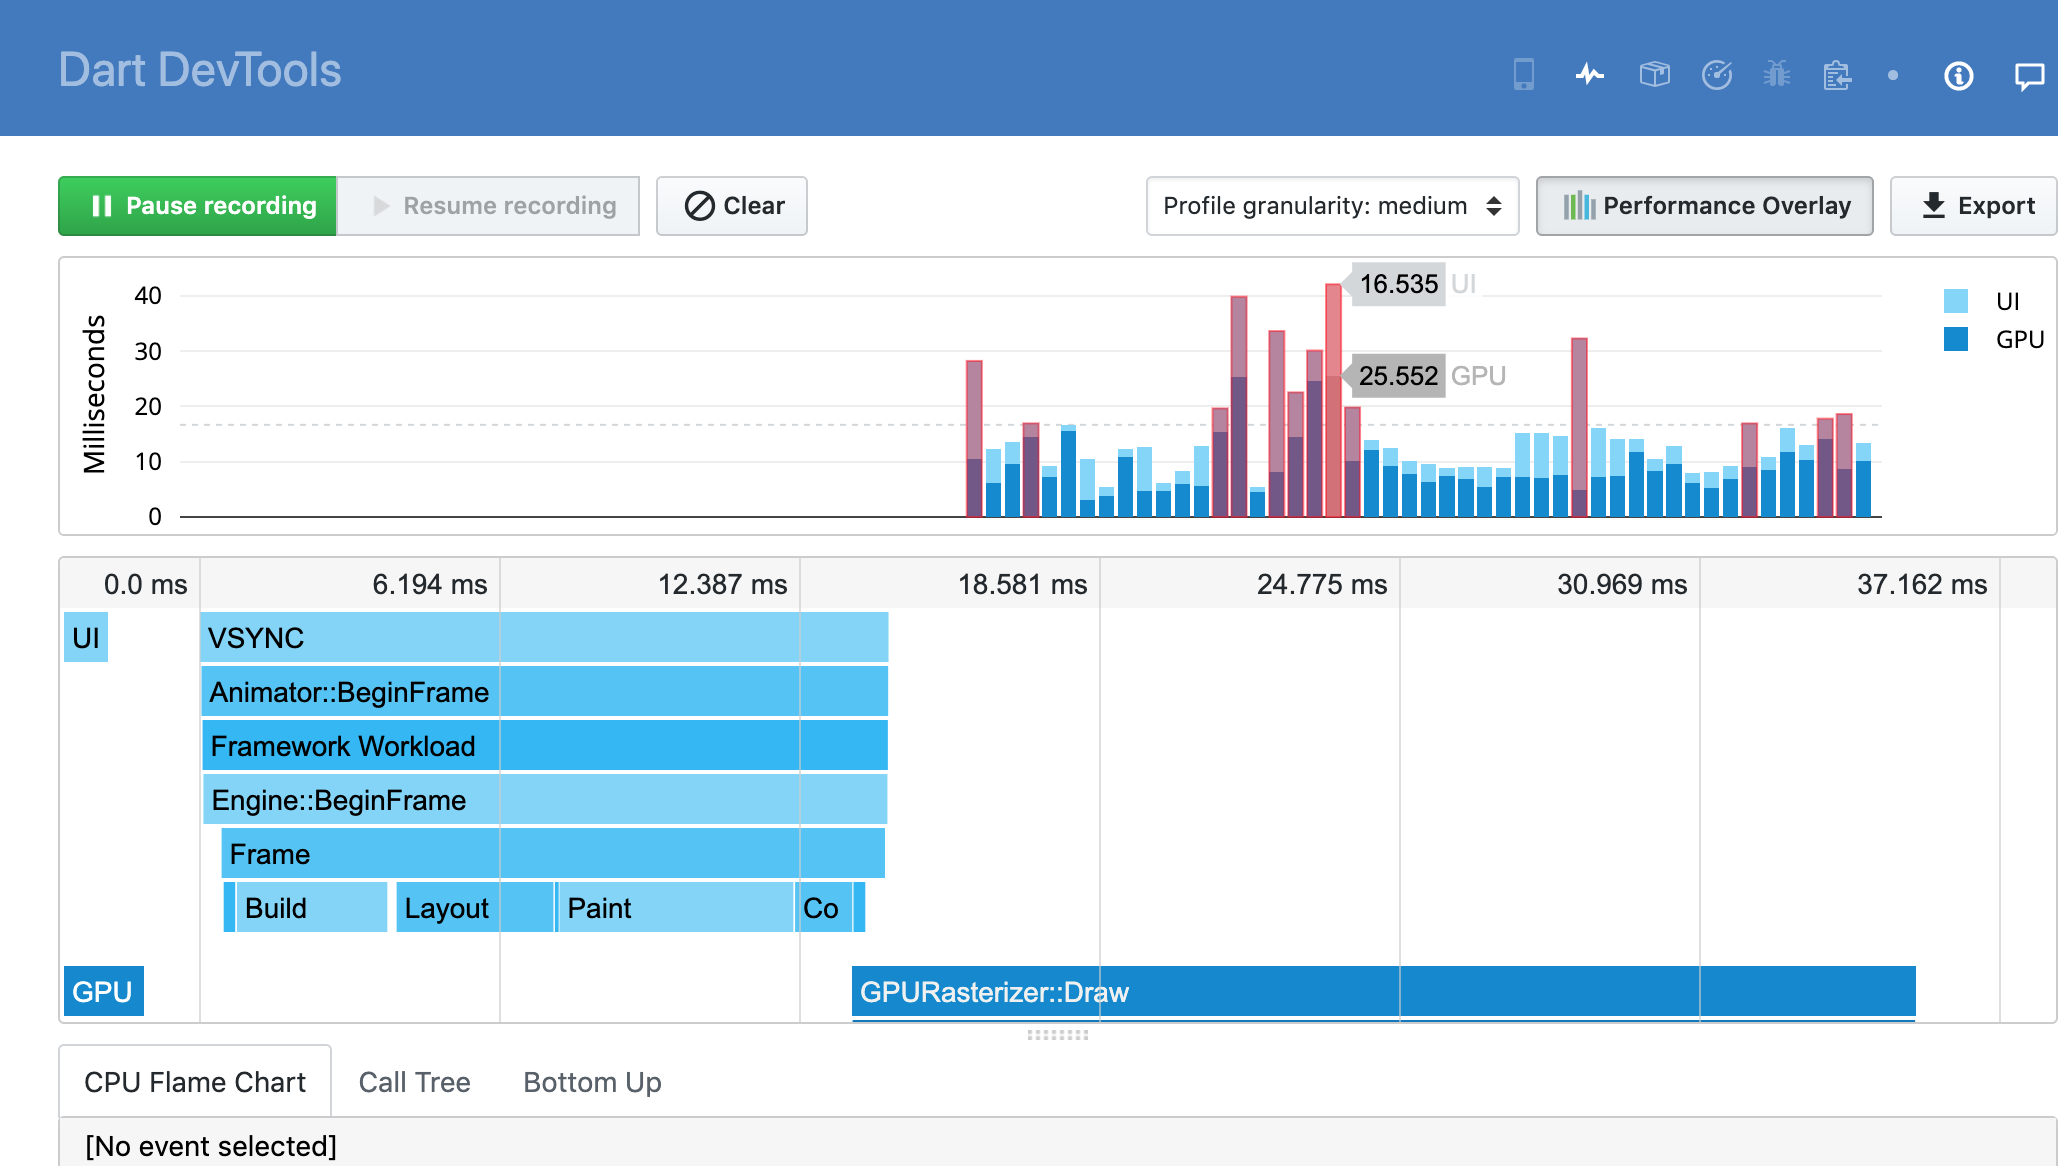
\includegraphics[keepaspectratio,alt={Dart dev tools}]{images/dart_devtools.png}}
\caption{Dart dev tools}
\end{figure}

很可惜从这个分析结果中我没有能找到对我有帮助的信息，唯一只能说确定的确会卡顿\ldots{}

\subsection{换个思路继续试}\label{ux6362ux4e2aux601dux8defux7ee7ux7eedux8bd5}

因为从这条路感觉已经走不通了，所以决定从其他的地方入手继续查。我注意到在登录的时候，偶尔会出现这样的日志：

\begin{verbatim}
I/Choreographer(15562): Skipped 107 frames!  The application may be doing too much work on its main thread.
\end{verbatim}

这说明啥？说明的确是卡了\ldots.这时候我开始怀疑，如果在登录这个事件里面做的事情很多的情况下，即便我们用了async/await，是不是也会卡顿呢？为了屏蔽掉其他条件的干扰，我们需要将登陆事件变得简单一些：

\begin{Shaded}
\begin{Highlighting}[]
\NormalTok{oid onPasswordSubmitted(BuildContext context}\OperatorTok{,} \DataTypeTok{String}\NormalTok{ password) }\AttributeTok{async} \OperatorTok{\{}
\NormalTok{  print(}\StringTok{\textquotesingle{}login with: $\{password\}\textquotesingle{}}\NormalTok{);}
  \ControlFlowTok{for}\NormalTok{(}\DataTypeTok{int}\NormalTok{ i }\OperatorTok{=} \DecValTok{0}\NormalTok{; i }\OperatorTok{\textless{}} \DecValTok{100000}\NormalTok{; i}\OperatorTok{++}\NormalTok{) }\OperatorTok{\{}
  \OperatorTok{\}}
\OperatorTok{\}}
\end{Highlighting}
\end{Shaded}

果然发现这样UI一样会卡住，甚至卡的更厉害了，根本连进度圈都出不来了。从这个结果来看，说明async/await并不能保证不会block住UI，顺着这个思路朝下找，于是就找到问题的根本原因了。

\section{让事件在单独的线程中运行}\label{ux8ba9ux4e8bux4ef6ux5728ux5355ux72ecux7684ux7ebfux7a0bux4e2dux8fd0ux884c}

\subsection{Flutter线程模型}\label{flutterux7ebfux7a0bux6a21ux578b}

原来dart跟JavaScript一样是一个单线程的模型，也就是是说，async/await里面的方法并不是在多个线程中取执行的，而是通过事件机制，在单线程中完成的。那么就很容易解释UI卡顿的场景了，UI更新和事件代码是交替执行的，如果其中事件执行的部分花费了较长时间，UI就没办法去更新，所以界面就会卡在那里，也就是日志里面所说的\texttt{Skipped\ 107\ frames!\ \ The\ application\ may\ be\ doing\ too\ much\ work\ on\ its\ main\ thread.}了。

\begin{figure}
\centering
\pandocbounded{\includegraphics[keepaspectratio,alt={Dart event model}]{https://cdn.jsdelivr.net/gh/flutterchina/flutter-in-action/docs/imgs/2-12.png}}
\caption{Dart event model}
\end{figure}

从dart的文档中可以了解到，dart内部有两个队列：

\begin{itemize}
\tightlist
\item
  event queue： 包含所有的外部事件例如IO、点击、绘制等
\item
  microtask queue： 微任务通常来自于dart内部或者手动插入\texttt{Future.microtask(…)}
\end{itemize}

microstask队列的优先级是要高于事件队列的。这里我们的登录事件和UI更新都同在事件队列中，很显然是因为我们的登录事件耗时太长从而掉帧了，那么解决的方案也就是，可不可以在新的线程中执行我们的事件呢？

\subsection{Isolate机制}\label{isolateux673aux5236}

研究了一下发现在dart中不叫线程，如果想达到这种目的需要使用一个称之为\texttt{Isolate}的东西，大致相当于新开一个线程来处理。要使用Isolate有两种办法：

\begin{itemize}
\tightlist
\item
  使用\texttt{compute}方法
\item
  使用\texttt{Isolate.spawn}（更低级的操作）
\end{itemize}

下面是一个例子：

\begin{Shaded}
\begin{Highlighting}[]
\DataTypeTok{Future}\OperatorTok{\textless{}}\DataTypeTok{List}\OperatorTok{\textless{}}\NormalTok{Photo}\OperatorTok{\textgreater{}\textgreater{}}\NormalTok{ fetchPhotos(http}\OperatorTok{.}\NormalTok{Client client) }\AttributeTok{async} \OperatorTok{\{}
  \AttributeTok{final}\NormalTok{ response }\OperatorTok{=}
      \AttributeTok{await}\NormalTok{ client}\OperatorTok{.}\KeywordTok{get}\NormalTok{(}\StringTok{\textquotesingle{}https://jsonplaceholder.typicode.com/photos\textquotesingle{}}\NormalTok{);}

  \CommentTok{// Use the compute function to run parsePhotos in a separate isolate.}
  \KeywordTok{return}\NormalTok{ compute(parsePhotos}\OperatorTok{,}\NormalTok{ response}\OperatorTok{.}\NormalTok{body);}
\OperatorTok{\}}
\end{Highlighting}
\end{Shaded}

\subsection{Compute方法}\label{computeux65b9ux6cd5}

看样子使用Isolate看似就像在Java中新建一个线程一样，然后就可以在线程中运行代码了。那我们直接把登录事件的处理挪进去不就得了么？然而实际情况是，这玩意并不是十分好用，有着诸多（恶心）的限制。先来看一下最简单直接的\texttt{compute}方法：

\begin{Shaded}
\begin{Highlighting}[]
\KeywordTok{typedef}\NormalTok{ ComputeCallback}\OperatorTok{\textless{}}\NormalTok{Q}\OperatorTok{,}\NormalTok{ R}\OperatorTok{\textgreater{}} \OperatorTok{=}\NormalTok{ FutureOr}\OperatorTok{\textless{}}\NormalTok{R}\OperatorTok{\textgreater{}} \KeywordTok{Function}\NormalTok{(Q message);}
\end{Highlighting}
\end{Shaded}

这个方法有两个参数，一个是callback（相当于java中的Runnable，就是你要执行的方法)，另一个是message，相当于是参数。这些参数有着如下的限制：

\begin{itemize}
\tightlist
\item
  callback必须是顶级的方法或者\texttt{static}方法，不能是类的实例方法或者是闭包
\item
  只有一个参数，那么我的方法需要传多个参数怎么办？
\end{itemize}

这就有些尴尬了，不仅要求是静态方法，还限制了参数，而我们的事件处理中有很多的依赖项，这可咋放进去呢？那么很可能只能用另一种方式了。

\subsection{Isolate.spawn}\label{isolate.spawn}

这个就显得更为麻烦了，大致的用法是这样的：

\begin{Shaded}
\begin{Highlighting}[]

\DataTypeTok{var}\NormalTok{ ourFirstReceivePort }\OperatorTok{=} \KeywordTok{new}\NormalTok{ ReceivePort();             }\CommentTok{// 需要一个ReceivePort来接收消息}
\AttributeTok{await}\NormalTok{ Isolate}\OperatorTok{.}\NormalTok{spawn(echo}\OperatorTok{,}\NormalTok{ ourFirstReceivePort}\OperatorTok{.}\NormalTok{sendPort); }\CommentTok{// 创建一个Isolate}
\DataTypeTok{var}\NormalTok{ echoPort }\OperatorTok{=} \AttributeTok{await}\NormalTok{ ourFirstReceivePort}\OperatorTok{.}\NormalTok{first;          }\CommentTok{// 等待执行完成并接收返回值}

\CommentTok{// 在Isolate中运行的代码需要将返回值通过sendPort发送过来}
\NormalTok{sendPort}\OperatorTok{.}\NormalTok{send(}\OperatorTok{...}\NormalTok{);}
\end{Highlighting}
\end{Shaded}

这个\texttt{spawn}方法如下：

\begin{Shaded}
\begin{Highlighting}[]
\KeywordTok{external} \AttributeTok{static} \DataTypeTok{Future}\OperatorTok{\textless{}}\NormalTok{Isolate}\OperatorTok{\textgreater{}}\NormalTok{ spawn}\OperatorTok{\textless{}}\NormalTok{T}\OperatorTok{\textgreater{}}\NormalTok{(}
      \DataTypeTok{void}\NormalTok{ entryPoint(T message)}\OperatorTok{,}\NormalTok{ T message}\OperatorTok{,}
      \OperatorTok{\{}\DataTypeTok{bool}\NormalTok{ paused}\OperatorTok{:} \ConstantTok{false}\OperatorTok{,}
      \DataTypeTok{bool}\NormalTok{ errorsAreFatal}\OperatorTok{,}
\NormalTok{      SendPort onExit}\OperatorTok{,}
\NormalTok{      SendPort onError}\OperatorTok{,}
\NormalTok{      @Since(}\StringTok{"2.3"}\NormalTok{) }\DataTypeTok{String}\NormalTok{ debugName}\OperatorTok{\}}\NormalTok{);}
\end{Highlighting}
\end{Shaded}

同样有着如下的限制：

\begin{itemize}
\tightlist
\item
  两个参数，一个entryPoint，另一个是这个entryPoint方法的唯一参数（也就是message)
\item
  entryPoint方法必须是顶级方法或者静态方法
\item
  message参数必须是基本类型、SendPort或者只包含这两者的list或者map。
\end{itemize}

这样就更加有些尴尬了，如果我们希望调用一个实例方法怎么办呢？我的登录过程中的一个关键步骤是调用argon2，这个方法我希望能在单独的线程之中调用：

\begin{Shaded}
\begin{Highlighting}[]
\KeywordTok{class}\NormalTok{ Argon2Kdf }\KeywordTok{implements}\NormalTok{ Kdf }\OperatorTok{\{}
  \KeywordTok{@override}
  \DataTypeTok{Future}\OperatorTok{\textless{}}\NormalTok{Uint8List}\OperatorTok{\textgreater{}}\NormalTok{ derive(Uint8List password}\OperatorTok{,}\NormalTok{ Uint8List salt) }\AttributeTok{async} \OperatorTok{\{}
\NormalTok{    Argon2 argon2 }\OperatorTok{=} \KeywordTok{new}\NormalTok{ Argon2();}
    \KeywordTok{return} \AttributeTok{await}\NormalTok{ argon2}\OperatorTok{.}\NormalTok{argon2i(password}\OperatorTok{,}\NormalTok{ salt) }\KeywordTok{as}\NormalTok{ Uint8List;}
  \OperatorTok{\}}
\OperatorTok{\}}
\end{Highlighting}
\end{Shaded}

这个方法本身是一个实例方法，既然我们只能用顶级方法和实例方法，而且Argon2这个类也没有什么依赖，也罢，那就创建一个好了，没有问题，现在问题来了，我们需要的两个参数是password和salt，这个参数类型不是基本类型，不支持呢，咋办呢？

\subsection{Isolate中通信}\label{isolateux4e2dux901aux4fe1}

原来isolate不像Java的线程一样可以使用共享内存，而是想actor模型一样，只能通过消息进行通信。那么，我们需要将参数转换为支持的基本类型，通过SendPort发送过去：

\begin{Shaded}
\begin{Highlighting}[]
\KeywordTok{class}\NormalTok{ Argon2Kdf }\KeywordTok{implements}\NormalTok{ Kdf }\OperatorTok{\{}
  \AttributeTok{static} \AttributeTok{final}\NormalTok{ Argon2 argon2 }\OperatorTok{=}\NormalTok{ Argon2(iterations}\OperatorTok{:} \DecValTok{2}\NormalTok{);}

  \AttributeTok{static} \DataTypeTok{void}\NormalTok{ argon2Call(SendPort replyPort) }\AttributeTok{async} \OperatorTok{\{}
    \AttributeTok{final}\NormalTok{ receivePort }\OperatorTok{=}\NormalTok{ ReceivePort();}
\NormalTok{    replyPort}\OperatorTok{.}\NormalTok{send(receivePort}\OperatorTok{.}\NormalTok{sendPort);}
    \AttributeTok{final} \DataTypeTok{List}\OperatorTok{\textless{}}\AttributeTok{dynamic}\OperatorTok{\textgreater{}}\NormalTok{ params }\OperatorTok{=} \AttributeTok{await}\NormalTok{ receivePort}\OperatorTok{.}\NormalTok{first;}
    \AttributeTok{final}\NormalTok{ SendPort reportPort1 }\OperatorTok{=}\NormalTok{ params[}\DecValTok{0}\NormalTok{];}

    \AttributeTok{final} \DataTypeTok{String}\NormalTok{ passwordHex }\OperatorTok{=}\NormalTok{ params[}\DecValTok{1}\NormalTok{];}
    \AttributeTok{final} \DataTypeTok{String}\NormalTok{ saltHex }\OperatorTok{=}\NormalTok{ params[}\DecValTok{2}\NormalTok{];}
    \AttributeTok{final}\NormalTok{ Uint8List password }\OperatorTok{=}\NormalTok{ hex}\OperatorTok{.}\NormalTok{decode(passwordHex) }\KeywordTok{as}\NormalTok{ Uint8List;}
    \AttributeTok{final}\NormalTok{ Uint8List salt }\OperatorTok{=}\NormalTok{ hex}\OperatorTok{.}\NormalTok{decode(saltHex) }\KeywordTok{as}\NormalTok{ Uint8List;}

    \AttributeTok{final}\NormalTok{ Uint8List result }\OperatorTok{=} \AttributeTok{await}\NormalTok{ argon2}\OperatorTok{.}\NormalTok{argon2i(password}\OperatorTok{,}\NormalTok{ salt) }\KeywordTok{as}\NormalTok{ Uint8List;}

\NormalTok{    reportPort1}\OperatorTok{.}\NormalTok{send(hex}\OperatorTok{.}\NormalTok{encode(result));}
  \OperatorTok{\}}

  \KeywordTok{@override}
  \DataTypeTok{Future}\OperatorTok{\textless{}}\NormalTok{Uint8List}\OperatorTok{\textgreater{}}\NormalTok{ derive(Uint8List password}\OperatorTok{,}\NormalTok{ Uint8List salt) }\AttributeTok{async} \OperatorTok{\{}
    \AttributeTok{final}\NormalTok{ ReceivePort response }\OperatorTok{=}\NormalTok{ ReceivePort();}
    \AttributeTok{final}\NormalTok{ isolate }\OperatorTok{=} \AttributeTok{await}\NormalTok{ FlutterIsolate}\OperatorTok{.}\NormalTok{spawn(argon2Call}\OperatorTok{,}\NormalTok{ response}\OperatorTok{.}\NormalTok{sendPort);}
    \AttributeTok{final}\NormalTok{ SendPort sendPort }\OperatorTok{=} \AttributeTok{await}\NormalTok{ response}\OperatorTok{.}\NormalTok{first;}
    \AttributeTok{final}\NormalTok{ ReceivePort response1 }\OperatorTok{=}\NormalTok{ ReceivePort();}
\NormalTok{    sendPort}\OperatorTok{.}\NormalTok{send([response1}\OperatorTok{.}\NormalTok{sendPort}\OperatorTok{,}\NormalTok{ hex}\OperatorTok{.}\NormalTok{encode(password)}\OperatorTok{,}\NormalTok{ hex}\OperatorTok{.}\NormalTok{encode(salt)]);}
    \AttributeTok{final} \DataTypeTok{String}\NormalTok{ result }\OperatorTok{=} \AttributeTok{await}\NormalTok{ response1}\OperatorTok{.}\NormalTok{first;}

\NormalTok{    isolate}\OperatorTok{.}\NormalTok{kill();}

    \KeywordTok{return}\NormalTok{ hex}\OperatorTok{.}\NormalTok{decode(result);}
  \OperatorTok{\}}
\OperatorTok{\}}
\end{Highlighting}
\end{Shaded}

这里有两点需要注意：

\begin{itemize}
\tightlist
\item
  调用\texttt{await\ response.first}之后这个SendPort就自动解除订阅了，不能用来接收其他消息了
\item
  Isolate.spawn不支持运行插件代码，所以用FlutterIsolate这个库来实现，而使用方法是一致的
\end{itemize}

如果直接使用\texttt{Isolate.spawn}会有如下的报错信息:

\begin{verbatim}
E/flutter (18071): [ERROR:flutter/runtime/dart_isolate.cc(808)] Unhandled exception:
E/flutter (18071): error: native function 'Window_sendPlatformMessage' (4 arguments) cannot be found
\end{verbatim}

这样最终的效果就是:

\begin{figure}
\centering
\pandocbounded{\includegraphics[keepaspectratio,alt={Login unblocked}]{images/login_unblocked.gif}}
\caption{Login unblocked}
\end{figure}

\begin{itemize}
\tightlist
\item
  \href{https://medium.com/dartlang/dart-asynchronous-programming-isolates-and-event-loops-bffc3e296a6a}{Dart asynchronous programming: Isolates and event loops}
\item
  \href{https://flutter.dev/docs/cookbook/networking/background-parsing\#4-move-this-work-to-a-separate-isolate}{Move this work to a separate isolate}
\item
  \href{https://pub.dev/packages/flutter_isolate}{flutter\_isolate}
\item
  \href{https://alvinalexander.com/dart/dart-isolates-example}{A Dart Isolates example (Actors in Dart)}
\item
  \href{https://github.com/flutter/flutter/issues/26413}{`Window\_sendPlatformMessage' (4 arguments) cannot be found}
\item
  \href{https://stackoverflow.com/questions/54127158/flutter-window-sendplatformmessage-4-arguments-cannot-be-found}{Flutter - `Window\_sendPlatformMessage' (4 arguments) cannot be found}
\item
  \href{https://github.com/dart-lang/sdk/issues/35962}{Cannot send regular Dart Instance to Isolate spawned with spawnUri}
\item
  \href{https://github.com/flutter/flutter/issues/34993}{Plugins crash with ``Methods marked with @UiThread must be executed on the main thread.''}
\item
  \href{https://book.flutterchina.club/chapter2/thread_model_and_error_report.html}{Dart单线程模型}
\end{itemize}


\end{document}
